\chapter{Flow through a hole -- determining the acoustic impedance} 

\modinfo{Directory}{FlowResistance}
\modinfo{Solvers}{\Idx{FlowSolve}}
\modinfo{Tools}{\Idx{ElmerGrid}, editor}
\modinfo{Dimensions}{3D, Steady-state}

\noindent
Note: This test case is available as consistency tests 
\texttt{FlowResNoslip} and \texttt{FlowResSlip}. This may be outdated
in parts. For example, it is not necessary to use any special unit system,
and also the computation of forces is now more accurate.

\subsection*{Case definition}

The problem at hand consists of finding the resistance that a fluid
faces as it is forced to flow through a hole. The flow resistance is
stated by the ratio of pressure drop over the hole and the input
velocity. In micro-system modeling, the hole resistance is often needed
to analyse the gas damping effect in perforated structures. Here, the
contribution of the holes is homogenized over the perforated structure
based on a single hole resistance. For homogenization in Elmer, the
specific \Idx{acoustic impedance} is used to represent the flow
resistance. Specific acoustic impedance $z_h$ is defined as
\begin{equation}
z_h = \frac{p}{v} = \frac{F}{vA_h},
\end{equation}
where $F$ is the net force due to gas on the moving surface, $v$ is
the velocity of the gas on the same surface, and $A_h$ is the area of
the moving surface. The calculation is best performed in a unit cell
of the geometry.

In order to the homogenization to be possible, the dependence of input
velocity and the net force should be linear. Further, there should not
be a phase change between these two quantities. These conditions are
satisfied when the flow is incompressible.  In a linear case, the
fluid flow can be treated with the linear form of Navier-Stokes
equations called the \Idx{Stokes equation}
\begin{equation}
\rho\frac{\partial \vec{u}}{\partial t}
-\nabla\cdot(2\eta\overline{\overline{\varepsilon}}) +\nabla p =
\rho \vec{f},
\end{equation}
where $\vec{u}$ is the unknown velocity field, $p$ is the pressure,
$\eta$ is the viscosity of the fluid, $\rho\vec{f}$ is a body force
and $\overline{\overline{\varepsilon}}$ is the linearised strain
tensor. Note, that the stationary version of the above equation can be
used in homogenization calculations.

The condition for Stokes equation to apply is that the Reynolds number
$Re$ of the problem should be small
\begin{equation}
Re = \frac{\rho UL}{\eta},
\end{equation}
where $\rho$ is density of the fluid and $U$ and $L$ are,
respectively, the velocity and length scales of the problem.

The issue of compressibility is more difficult to answer. A classical
condition for the compressibility is that the Mach number $Ma$ of the
problem should be small
\begin{equation}
Ma = \frac{U}{a} < 0.3,
\end{equation}
where $a$ is the speed of sound in the gas in operating conditions and
the value~0.3 is often stated limit for a small Mach number (actually,
the condition is that $Ma^2$ has to be small).  Also the frequency and
amplitude of the oscillations of the system have an effect on the
validity of the linearity and incompressibility assumptions, since
they affect the velocity scale of the problem.

However, also other factors have an effect on the compressibility of
the gas. In micro-systems, the viscous effects on pressure, or even
temperature changes, can affect the density of the gas. A
condition for viscous pressure changes is that $Ma^2/Re$ has to be
small, and for temperature, in addition, that the Prandtl number $Pr$
may not be too large
\begin{equation}
Pr = \frac{\eta c_p}{k},
\end{equation}
where $c_p$ is the heat capacity ({\em ie.} specific heat) in constant
pressure and $k$ is the thermal conductivity.

The conditions listed here for the flow to be approximately
incompressible are only an overview and the validity of
incompressibility assumption should be considered in each case
separately. In micro-systems, refer for example to the article
M.~Gad-el-Hak, J.~Fluids Eng., 121, 5--33, 1999. Additionally, it is
advisable to perform numerical checks on the issue.

One final point on the applicability of the Stokes (or Navier-Stokes)
equations is the effect of gas rarefaction. If the dimensions of the
problem are very small the continuity assumption may not be valid
anymore. The importance of the gas rarefaction effects are given by
the Knudsen number $Kn$
\begin{equation}
Kn = \frac{{\cal L}}{L},
\end{equation}
where ${\cal L}$ is the mean free path of the gas molecules. The mean
free path depends inversely on ambient pressure, which has to take
into account in stating the Knudsen number. For Knudsen numbers close
to and less than~1, slip boundary conditions should be used.

To summarize, the motivation of this tutorial is to perform a linear
incompressible simulation of fluid flowing through a hole. The wake
for the flow is a constant velocity boundary condition for a boundary
before the hole. On the same boundary, the force caused by the fluid
is recorded. These two quantities can then be used to determine the
specific acoustic impedance of a single hole. The constant velocity
boundary condition may be interpreted as describing a moving wall with
small displacement. In this particular tutorial, a symmetrical
quadrant of a square-shaped hole is used.



\subsection*{Solution procedure}

The solution for the problem is found by solving iteratively the
Stokes equation. Nonlinear iterations are not needed, since the
problem is linear.

The computational mesh should include enough free space after the hole
so that any artificial effects due to the boundaries of the mesh are
avoided. In this tutorial, the geometry is created and meshed using
the ElmerGrid program by the command
{\tt
elmergrid 1 2 hole.grd}. 
The default mesh consists of about 12000 nodes and 10500 eight-noded
hexahedrons.

The header section of solver input file includes only the location of
the mesh files.
\ttbegin
Header
  Mesh DB "." "hole"
End
\ttend

In the simulation section, a steady-state three-dimensional analysis
is defined.
\ttbegin
Simulation
  Coordinate System = Cartesian 3D
  Simulation Type = Steady State
  Steady State Max Iterations = 1
  Output File = "flow.result"
  Post File = "flow.vtu"
End
\ttend

The geometry contains only one body and no body forces or initial
conditions are present. The body section reads thus as follows.
\ttbegin
Body 1
  Equation = 1
  Material = 1
End
\ttend

For solving the flow patterns the Navier-Stokes solver is used but the
nonlinearity through convection is switched off in the equation block.
Also, solvers for the fluidic force and saving data are enabled.
\ttbegin
Equation 1
  Active Solvers(3) = Integer 1 2 3
  NS Convect = False
End
\ttend

Just a single iteration of the Navier-Stokes solver is needed, since
the equation is linear. This can be verified by switching the number
of nonlinear iterations to a value more than one, and observing the
change in solution between iteration steps.
\ttbegin
Solver 1
   Equation = Navier-Stokes
   Variable = Flow Solution
   Variable DOFs = 3
   Linear System Solver = Iterative
   Linear System Iterative Method = BiCGStab
   Linear System Preconditioning = ILU0
   Linear System Max Iterations = 200
   Linear System Convergence Tolerance = 1.0e-08
   Stabilize = True
   Nonlinear System Convergence Tolerance = 1.0e-05
   Nonlinear System Max Iterations = 1
   Nonlinear System Newton After Iterations = 3
   Nonlinear System Newton After Tolerance = 1.0e-08
   Nonlinear System Relaxation Factor = 1.0
   Steady State Convergence Tolerance = 1.0e-05
End
\ttend

The fluidic force solver needs to be run only once, after the flow
solution is finished. With the keyword {\tt Calculate Viscous Force} it
is possible to define whether the viscous forces of the fluid are
included in the force or not. If this is set to false, only the
pressure integral is calculated.
\ttbegin
Solver 2
  Exec Solver = After All
  Equation = Fluidic Force
  Procedure  ="FluidicForce" "ForceCompute"
  Calculate Viscous Force = True
End
\ttend

The final solver is used to save data from the analysis. With the
following definitions, the input velocity and the net force on the
input boundary as well as the area of the boundary are written into a
file called {\tt flowdata.dat}.
\ttbegin
Solver 3
  Exec Solver = After All
  Equation = SaveScalars
  Procedure = "\Idx{SaveData}" "SaveScalars"
  Filename = "flowdata.dat"
  Save Variable 1 = Velocity 3
  Save Coordinates(1,2) = 0.0 0.0
End
\ttend

The fluid is defined to be air. Note the Elmer \Idx{MEMS} units used.
\ttbegin
Material 1
  Name = Air
  Density = 1.293e-12
  Viscosity = 1.67e-5
End
\ttend

Finally, the boundary conditions. BC~1 defines the input boundary,
where also the fluidic force is calculated. BCs~2 and~4 define the
symmetry boundaries, BC~3 defines the no-slip conditions for the
walls, and BC~5 defines an open boundary.
\ttbegin
Boundary Condition 1
  Target Boundaries = 4
   Velocity 1 = 0.0
   Velocity 2 = 0.0
   Velocity 3 = 1.0e3
   Calculate Fluidic Force = True
End

Boundary Condition 2
  Target Boundaries(2) = 8 10
   Velocity 2 = 0.0
End

Boundary Condition 3
  Target Boundaries(4) = 1 2 3 7
   Velocity 1 = 0.0
   Velocity 2 = 0.0
   Velocity 3 = 0.0
End

Boundary Condition 4
  Target Boundaries(2) = 6 9
   Velocity 1 = 0.0
End

Boundary Condition 5
  Target Boundaries = 5
  Pressure = 0.0
End
\ttend

\subsection*{Slip boundary conditions}

The same simulation can also be performed using slip boundary
conditions. These are appropriate, as stated in introduction, when the
Knudsen number is between $10^{-3}$ and 1. The slip boundary condition
implemented in Elmer is of first order 
\begin{equation}
S\cdot \vec{u} = \overline{\overline{\sigma}}\cdot\vec{n},
\end{equation}
where $S$ is a vector containing the slip coefficients $s_i$ for each
velocity component, $\mu$ is the viscosity, and
$\overline{\overline{\sigma}}$ is the stress tensor. For Newtonian
fluids and for tangential directions of the boundary this gives
\begin{equation}
s_i u_i = \mu\frac{\partial u_i}{\partial n},
\end{equation}
where $s_i$ and $u_i$ refer to the same tangential component of the
slip coefficient and the flow velocity.

The value of the slip coefficient is related to the mean free path of
the gas molecules $\lambda$. For example, Maxwell's first order slip
boundary condition may be used (as in {\em e.g.} A.~Beskok, {\em
Num. Heat Transfer,} B, 40, 451--471, 2001):
\begin{equation}
u_i = \frac{2-\sigma_v}{\sigma_v}\lambda 
\frac{\partial u_i}{\partial n},
\end{equation}
where $\sigma_v$ is the tangential momentum accommodation coefficient,
which models the momentum exchange of gas molecules and the
surface. The accommodation coefficient is dependent on the gas and on
the surface, and recent measurements give a result of $\sigma_v\simeq
0.80$ for various monoatomic gases such as Argon in contact with
prime Silicon crystal. 

The slip coefficient of Elmer can finally be written as
\begin{equation}
s_i = \frac{\mu}{\lambda}\frac{\sigma_v}{2-\sigma_v}.
\end{equation}
The mean free path is defined as
\begin{equation}
\lambda = \frac{\mu}{\rho}\sqrt{\frac{\pi M}{2RT}}_,
\end{equation}
where $\rho$ is density, $M$ is the molar mass, $T$ is the
temperature, and $R=8.3145$~J/mol~K is the molar gas constant.

In the Elmer analysis, only a few changes in the sif-file are needed
to make the slip conditions active. The flow force boundary conditions
have to be turned on and the numerical value of the slip coefficient
has to be defined on each boundary (here $s=$2e-4 is used for
air). Further below is a list of the Boundary Condition blocks. Note
that there are more BCs than in the no-slip simulation, since a
separate condition is needed for surfaces oriented differently in
space.

Generally, a normal-tangential orientation scheme for the boundary
conditions are needed, since the surfaces are not necessarily having a
normal vector pointing in one of the coordinate directions. This would
be done for each such boundary by the line
\ttbegin
  Normal-Tangential Velocity = True
\ttend
after which the Velocity component~1 points to the normal direction
and the other components to the tangential directions.

\ttbegin
! Definitions for slip boundary conditions:
Boundary Condition 1
  Target Boundaries = 4
   Flow Force BC = True
   Slip Coefficient 1 = 2e-4
   Slip Coefficient 2 = 2e-4
   Velocity 3 = 2.0e3
   Calculate Fluidic Force = True
End

Boundary Condition 2
  Target Boundaries(2) = 8 10
   Velocity 2 = 0.0
End

Boundary Condition 3
  Target Boundaries(2) = 2 3
   Flow Force BC = True
   Velocity 3 = 0.0
   Slip Coefficient 1 = 2e-4
   Slip Coefficient 2 = 2e-4
End

Boundary Condition 4
  Target Boundaries(2) = 6 9
   Velocity 1 = 0.0
End

Boundary Condition 5
  Target Boundaries = 5
  Pressure = 0.0
End

Boundary Condition 6
  Target Boundaries = 1
   Flow Force BC = True
   Velocity 1 = 0.0
   Slip Coefficient 2 = 2e-4
   Slip Coefficient 3 = 2e-4
End

Boundary Condition 7
  Target Boundaries = 7
   Flow Force BC = True
   Velocity 2 = 0.0
   Slip Coefficient 1 = 2e-4
   Slip Coefficient 3 = 2e-4
End
\ttend

\subsection*{Results}

The computation takes about 200~cpu seconds on an AlphaServer with
1~GHz central processor when trilinear elements are used (historical results).
The results
for two different input velocities taken from the file {\mbox{\tt
flowdata.dat}} are summarised in Table~\ref{tab:imped_res}. Also the
specific acoustic impedance $z_h$ is calculated in the table. The
results of slip and no-slip simulations are also compared.  Note that
for the force, only the component perpendicular to the surface should
be used since the other components cancel out due to symmetry. The
values in the table are again given in Elmer MEMS units (these units
are numerically favourable in small dimensions and were used historically
in MEMS projects).
\begin{table}[htb]
\caption{Results of flow simulations for two input velocities}
\label{tab:imped_res}
\begin{center}
\begin{tabular}{cccc} \hline
$v$ & \ \ slip model\ \  & $F_z$ & $z_h$ \\ \hline 
$1.0\cdot 10^3$   & no-slip  & 36.13  &  $1.45\cdot10^{-3}$ \\
$2.0\cdot 10^3$   & no-slip  & 72.25  &  $1.45\cdot10^{-3}$ \\ \hline
$1.0\cdot 10^3$   & slip     & 29.30  &  $1.17\cdot10^{-3}$ \\
$2.0\cdot 10^3$   & slip     & 58.60  &  $1.17\cdot10^{-3}$ \\ \hline
\end{tabular}
\end{center}
\end{table}

The identical values obtained for the spesific acoustic impedance in
Table~\ref{tab:imped_res} prove by no means that the flow in reality
is linear, since this was the assumption and the simulation performed
can and should not reveal any nonlinear behavior. The results
indicate, though, that allowing slip on the boundaries reduces the
resistance that the fluid faces. This example shows that in
micro-systems, as the dimension of the smallest flow channel is in the
range of a micrometer, it is reasonable to use slip boundary
conditions for the velocity.

\begin{figure}[htb]
  \centerline{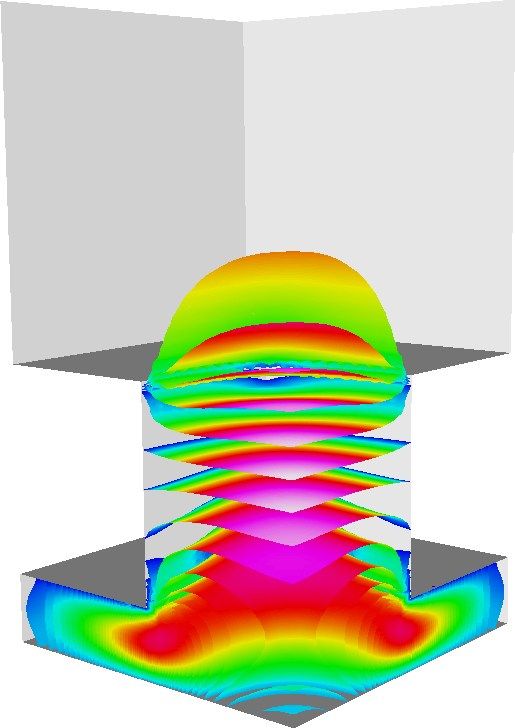
\includegraphics[width=0.40\textwidth]{flow_res}}
  \caption{The linear flow results.} 
  \label{fig:flow_res}
\end{figure}
Finally, a picture of the results obtained with no-slip conditions is
presented. The Fig.~\ref{fig:flow_res} shows a lot of pressure
isosurfaces which are coloured using the absolute value of the
velocity.

Note: it seems that the results with the current code are not
exactly the same. However, we didn't invest where the small discrepancy
might come from. 


\vfill
\mbox{}
